%%
%% This is file `sigconf.tex',
%% generated with the docstrip utility.
%%
%% The original source files were:
%%
%% samples.dtx  (with options: `sigconf')
%% 
%% IMPORTANT NOTICE:
%% 
%% For the copyright see the source file.
%% 
%% Any modified versions of this file must be renamed
%% with new filenames distinct from sample-sigconf.tex.
%% 
%% For distribution of the original source see the terms
%% for copying and modification in the file samples.dtx.
%% 
%% This generated file may be distributed as long as the
%% original source files, as listed above, are part of the
%% same distribution. (The sources need not necessarily be
%% in the same archive or directory.)
%%
%%
%% Commands for TeXCount
%TC:macro \cite [option:text,text]
%TC:macro \citep [option:text,text]
%TC:macro \citet [option:text,text]
%TC:envir table 0 1
%TC:envir table* 0 1
%TC:envir tabular [ignore] word
%TC:envir displaymath 0 word
%TC:envir math 0 word
%TC:envir comment 0 0
%%
%%
%% The first command in your LaTeX source must be the \documentclass command.
\documentclass[sigconf, pdftex]{acmart}
\usepackage{algorithmic, algorithm}
\usepackage{subfigure}
\usepackage{enumitem}

%%
%% \BibTeX command to typeset BibTeX logo in the docs
\AtBeginDocument{%
  \providecommand\BibTeX{{%
    Bib\TeX}}}

%% Rights management information.  This information is sent to you
%% when you complete the rights form.  These commands have SAMPLE
%% values in them; it is your responsibility as an author to replace
%% the commands and values with those provided to you when you
%% complete the rights form.
\setcopyright{acmcopyright}
\copyrightyear{2023}
\acmYear{2023}
\acmDOI{XXXXXXX.XXXXXXX}

%% These commands are for a PROCEEDINGS abstract or paper.
\acmConference[ACM xxxxx]{Make sure to enter the correct
  conference title from your rights confirmation emai}{April 01--04,
  2022}{City, State}
\acmPrice{15.00}
\acmISBN{978-1-4503-XXXX-X/18/06}


%%
%% Submission ID.
%% Use this when submitting an article to a sponsored event. You'll
%% receive a unique submission ID from the organizers
%% of the event, and this ID should be used as the parameter to this command.
%%\acmSubmissionID{123-A56-BU3}

%%
%% For managing citations, it is recommended to use bibliography
%% files in BibTeX format.
%%
%% You can then either use BibTeX with the ACM-Reference-Format style,
%% or BibLaTeX with the acmnumeric or acmauthoryear sytles, that include
%% support for advanced citation of software artefact from the
%% biblatex-software package, also separately available on CTAN.
%%
%% Look at the sample-*-biblatex.tex files for templates showcasing
%% the biblatex styles.
%%

%%
%% The majority of ACM publications use numbered citations and
%% references.  The command \citestyle{authoryear} switches to the
%% "author year" style.
%%
%% If you are preparing content for an event
%% sponsored by ACM SIGGRAPH, you must use the "author year" style of
%% citations and references.
%% Uncommenting
%% the next command will enable that style.
%%\citestyle{acmauthoryear}

%%
%% end of the preamble, start of the body of the document source.
\begin{document}


%%
%% The "title" command has an optional parameter,
%% allowing the author to define a "short title" to be used in page headers.
\title{Parrot: A Framework for Abstractive Summarization of Conversational Meetings}
	
%the Class Imbalance Problem in Medical Datasets}

%%
%% The "author" command and its associated commands are used to define
%% the authors and their affiliations.
%% Of note is the shared affiliation of the first two authors, and the
%% "authornote" and "authornotemark" commands
%% used to denote shared contribution to the research.
%
%\author{}
%\email{}
%\affiliation{%
%	\institution{}
%	\city{}
%	%	\state{WA}
%	\country{}
%}

\author{Vincent Marklynn }
%\authornote{Both authors contributed equally to this research.}
\email{vmarklynn@seattleu.edu}
%\orcid{1234-5678-9012}
\affiliation{%
	\institution{Seatle University}
%	\streetaddress{P.O. Box 1212}
	\city{Seattle}
	\state{WA}
	\country{USA}
%	\postcode{43017-6221}
}


\author{Anjali Sebastian}
\email{asebastian@seattleu.edu}
\affiliation{%
	\institution{Seattle University}
	% \streetaddress{Rono-Hills}
	\city{Seattle}
	\state{WA}
	\country{USA}
}

\author{Yong Long Tan }
\email{ytan@seattle.edu}
\affiliation{%
	\institution{Seattle University}
	% \streetaddress{Rono-Hills}
	\city{Seattle}
	\state{WA}
	\country{USA}
}

\author{Wan D. Bae}
\email{baew@seattleu.edu}
\affiliation{%
	\institution{Seattle University}
	% \streetaddress{Rono-Hills}
	\city{Seattle}
	\state{WA}
	\country{USA}
}

\author{Sada Narayanappa}
\email{sada.narayanappa@lmco.com}
\affiliation{%
	\institution{Lockheed Martin Spaces}
	%  \streetaddress{30 Shuangqing Rd}
	\city{Denver}
	\state{CO}
	\country{USA}
}



%%
%% By default, the full list of authors will be used in the page
%% headers. Often, this list is too long, and will overlap
%% other information printed in the page headers. This command allows
%% the author to define a more concise list
%% of authors' names for this purpose.
%\renewcommand{\shortauthors}{Bae et al.}

%%
%% The abstract is a short summary of the work to be presented in the
%% article.
\begin{abstract}
Around 83\% of employees spend a third of their workweek attending meetings. We aim to conduct analysis from speech to text specifically in conversations with more than two speakers in a meeting environment. Besides granting accessibility accommodations to hard-of-hearing people, we also want to provide accurate and insightful analysis to customers and researchers. With recent advances in automatic speech recognition and natural language processing models such as OpenAI’s Whisper and Meta’s BART, we seek to simplify the process of speech recognition and abstractive summarization of long meetings. Unlike extractive summarization, abstractive summarization creates summaries by synthesizing new words and sentences that maintain the original meaning of the source. This is challenging due to the necessity of NLP models for text generation. Our solution consists of developing a pipeline that takes large audio files (approximately 1 hour) and transcribes and diarizes the conversation using OpenAI’s Whisper and Pyannote. Our summarization solution involves retraining the BART model. Our retrained model makes the base-model compatible with summarizing long meeting dialogues and improves summarization by 148\% \textcolor{red}{(!!! should add results that show this number)}. The solution includes a front-end website built using Django that integrates our model and enables users to upload a meeting recording to get the full meeting transcript and summary.
\end{abstract}


%%
%% The code below is generated by the tool at http://dl.acm.org/ccs.cfm.
%% Please copy and paste the code instead of the example below.
%%
\begin{CCSXML}
<ccs2012>
 <concept>
  <concept_id>10010520.10010553.10010562</concept_id>
  <concept_desc>Computer systems organization~Embedded systems</concept_desc>
  <concept_significance>500</concept_significance>
 </concept>
 <concept>
  <concept_id>10010520.10010575.10010755</concept_id>
  <concept_desc>Computer systems organization~Redundancy</concept_desc>
  <concept_significance>300</concept_significance>
 </concept>
 <concept>
  <concept_id>10010520.10010553.10010554</concept_id>
  <concept_desc>Computer systems organization~Robotics</concept_desc>
  <concept_significance>100</concept_significance>
 </concept>
 <concept>
  <concept_id>10003033.10003083.10003095</concept_id>
  <concept_desc>Networks~Network reliability</concept_desc>
  <concept_significance>100</concept_significance>
 </concept>
</ccs2012>
\end{CCSXML}

\ccsdesc[500]{Computing methodologies~Machine learning algorithms}
\ccsdesc[500]{Applied computing~Document management and text processing}


%%
%% Keywords. The author(s) should pick words that accurately describe
%% the work being presented. Separate the keywords with commas.
\keywords{abstractive summarization, natural language generation, }
%% A "teaser" image appears between the author and affiliation
%% information and the body of the document, and typically spans the
%% page.
%\begin{teaserfigure}
%  \includegraphics[width=\textwidth]{sampleteaser}
%  \caption{Seattle Mariners at Spring Training, 2010.}
%  \Description{Enjoying the baseball game from the third-base
%  seats. Ichiro Suzuki preparing to bat.}
%  \label{fig:teaser}
%\end{teaserfigure}

%%
%% This command processes the author and affiliation and title
%% information and builds the first part of the formatted document.
\maketitle


\section{Introduction}
\label{sec:intro}
Meetings with multiple speakers can be challenging for individuals who require accessibility accommodations, such as hard-of-hearing people. Audio-to-text conversion has been a helpful tool to assist these individuals. Still, it does not address the issue of identifying the speaker in a meeting and generating a summary for the given meeting. Therefore, there is a need for a pipeline that can identify the speaker and summarize a given audio file. Besides granting accessibility accommodations to hard-of-hearing people, we also want to provide accurate and insightful analysis to customers and researchers, which can help them understand and utilize the content of the meetings better. In addition to providing accessibility accommodations for individuals who are hard of hearing, we want to offer precise and insightful analysis to both customers and researchers. This analysis can improve their comprehension and utilization of meeting content. This can be especially beneficial for organizations that need to monitor multiple meetings and extract key information for decision-making and research purposes.



\begin{figure*}[thbp]
	\centering
	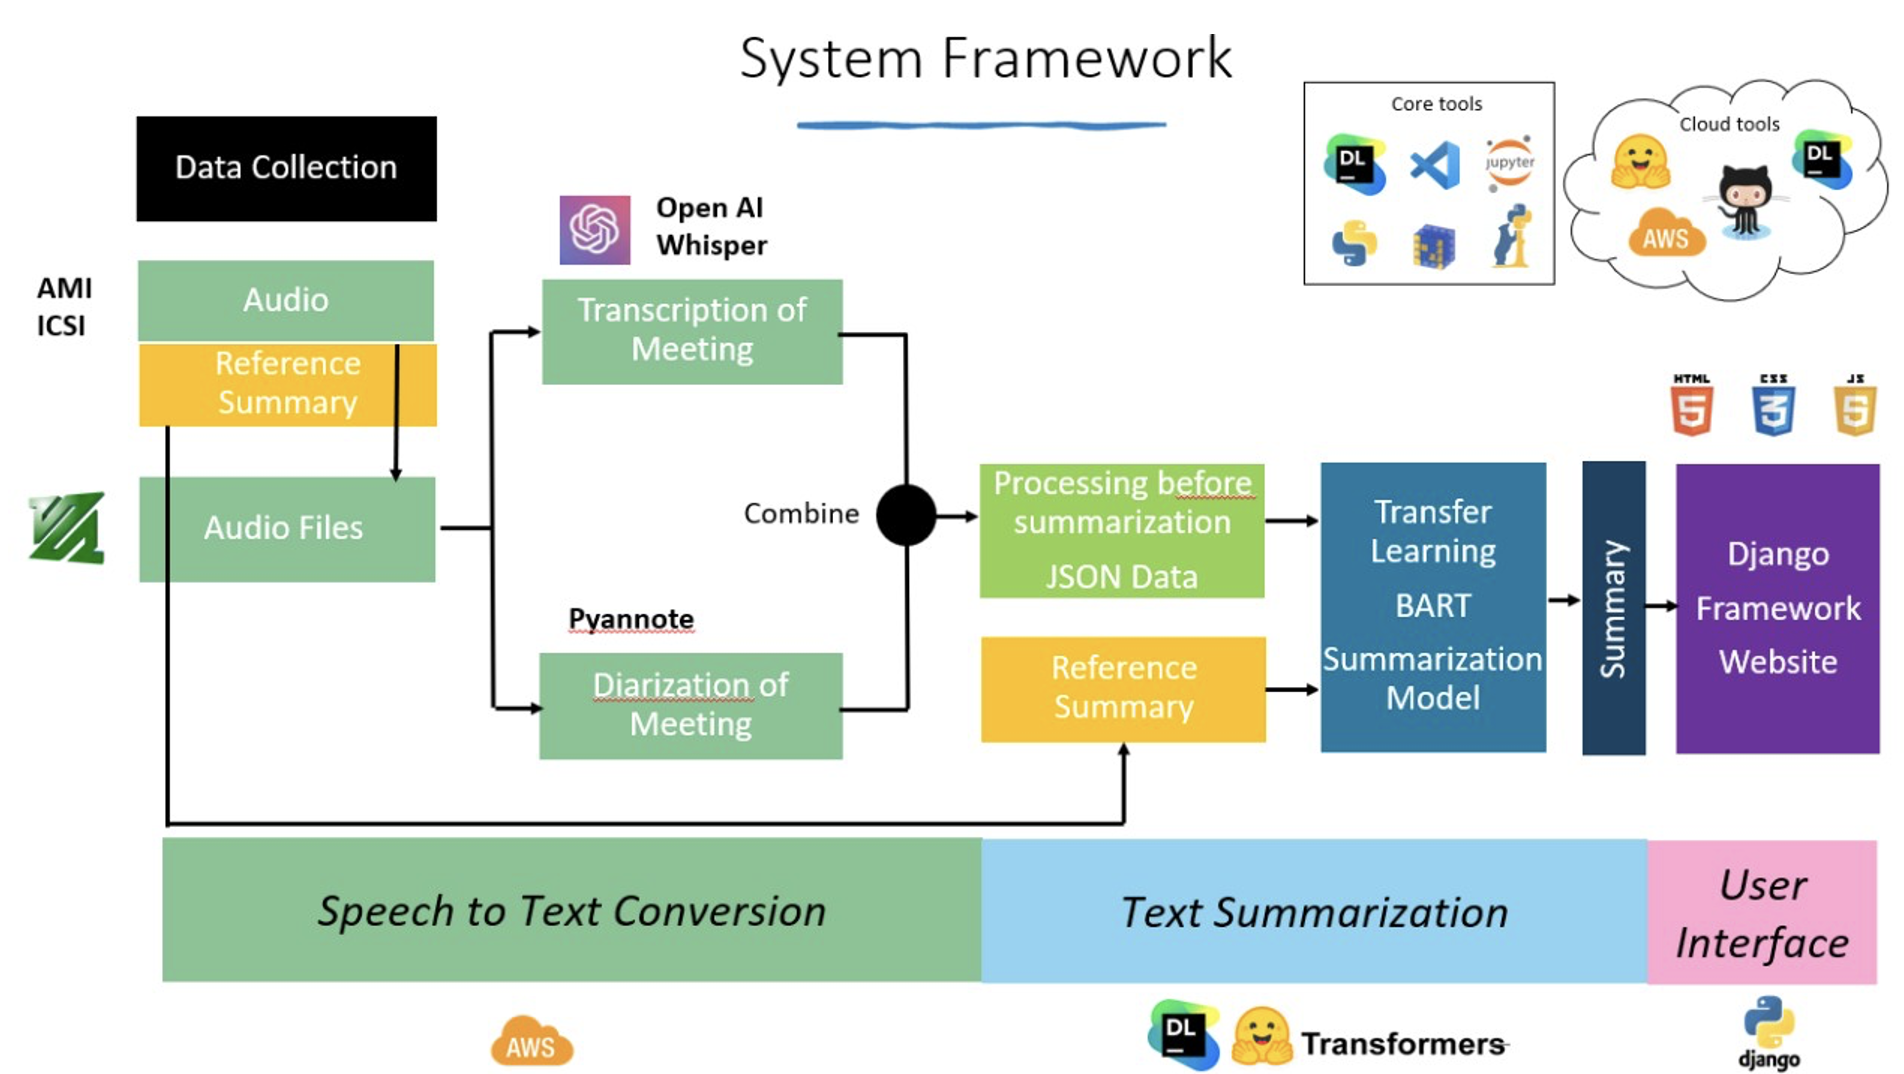
\includegraphics[width=14cm, height=6cm]{figures/overview}
	\caption{An overview of system framework}
	%\Description{Overview}
	\label{fig:overview}
	\textcolor{red}{will need to replace with a new figure. remove title and tool figures. reduce \# colors and bigger/clearer font}
\end{figure*}




We aim to conduct audio analysis from speech to text specifically in conversations with more than two speakers in a meeting environment. Besides granting accessibility accommodations to hard-of-hearing people, we also want to provide an accurate and insightful analysis for customers and researchers to leverage.

This audio analysis problem can be partitioned into four different parts:

\begin{itemize}
\item Automatic Transcription: We used OpenAI’s Whisper to automatically transcribe audio files.

\item Speaker Diarization: We used an opensource Python library called Pyannote to perform basic speaker diarization.

\item Summarization: We used a pre trained BART model trained on the CNN/Dailymail and SAMSUM datasets.

\item Visualization/Presentation: We developed a basic front-end web application where users can upload an audio file and receive a transcript and summary.

\end{itemize}

We created a working summarization pipeline starting with an Automatic Speaker Recognition (ASR) module consisting of OpenAI Whisper and Pyannote. For our summarization module, we performed transfer-learning on a pre trained BART sequence-to-sequence transformer model by training the model on a machine transcribed AMI/ICSI corpus to improve summarization for long meetings.



\section{Related Work}
\label{sec:related}
In recent years, the transformer encoder-decoder architecture has been widely used in the field of natural language processing (NLP). The essential compoents we integrated into our proposed framework are below. 

BART: Denoising sequence-to-sequence pre-training for natural language generation, translation, and comprehension \cite{bart}: BART is pretrained by corrupting the input text using some noise schemes and learning a model to reconstruct the original input. It reads the corrupted input in both directions, left to right or vice versa. The bidirectional encoder produces a set of hidden states that capture the meaning and context of our input text. Then, this collection of hidden states will get pushed to the autoregressive decoder. The decoder is another component that generates the output text one element at a time, where each element is conditioned on the previously generated elements.


QMSum \cite{zhong2021qmsum}: A new benchmark for query-based multi-domain meeting summarization. \textcolor{red}{A short summary of the paper's main ideas and contributions needs to be added. A New Benchmark for Query-based Multi-domain Meeting Summarization. QMSum is a novel benchmark designed for evaluating the performance of summarization models in the context of multi-domain meetings. This benchmark focuses on query-based summarization, which aims to generate concise summaries in response to specific user queries rather than generic summaries of entire meetings. QMSum contains a diverse collection of meeting transcripts, queries, and reference summaries, which helps facilitate the development and evaluation of more advanced, context-aware models for meeting summarization. For our work, we only reuse their reference summaries. These reference summaries will be used for evaluation, as we assume that they can be served as ground truth.}

\vspace{10mm}

Whisper \cite{radford2022robust}: \textcolor{red}{A short summary of the paper's main ideas and contributions needs to be added. Whisper is a system designed for automatic speech recognition, developed by OpenAI. It converts spoken language into written text using advanced speech recognition techniques. It has been trained on a vast dataset of multilingual and multitask supervised data gathered from the web. It is considered a state-of-the-art speech recognition system, providing highly accurate transcriptions promptly and outperforming many existing speech-to-text solutions. We utilize the base model version of Whisper and incorporate it into our system framework.}

\vspace{10mm}

Pyannote \cite{bredin2020pyannote}: \textcolor{red}{A short summary of the paper's main ideas and contributions needs to be added. Pyannote is a Python library that provides tools for various tasks in multimedia processing. We only utilize their speaker diarization tool to determine "who spoke when." Speaker diarization is the process of segmenting an audio stream into speaker-homogeneous sections. The Pyannote’s speaker diarization contribution lies in its open-source nature, fostering the continuous improvement and expansion of its capabilities. It facilitates effective and flexible audio segmentation into speaker-homogeneous sections.}
%Partitioning speakers (diarization) - Amazon Transcribe.
\vspace{10mm}

\textcolor{red}{***  A few reference papers are related to including audio summarization? Are there any work similar to our work? }



\section{Methods and Initial Analysis}
\label{sec:method}




\subsection{System Architecture Overview}
\label{sec:overview}

Our architecture can be separated into three parts:

\begin{enumerate}
\item Speech to Text Conversion: Using the AMI and ICSI corpus, we transcribed the audio files using Whisper. Next, we diarized the audio file using Pyannote and combined the two files into a single transcription.

\item Text Summarization: Using the human reference and the dataset that we have created we combined both to form a single JSON file. We then fed the JSON file into the pretrained BART model.

\item User Interface: Using the Django Framework, we created a simple web application that allows users to upload an audio file and receive a transcription and a summary of the meeting.
\end{enumerate}

The proposed pipeline is implemented in Python 3.8 using various tools. A complete list of tools we used as follows: BART \textcolor{red}{[open source code cite?]}, FFMEG \cite{FFmpeg}, Whisper Open AI \cite{whisper}, Pyannote \cite{pyannotewhisper}, Hugging Face Transformers \textcolor{red}{[open source code cite?]}, and Django \cite{Django} . 

%\cite{whisper, } are used with speaker diarization where the audio is partitioned into segments to identify speakers.  




\subsection{Speech to Text Conversion}
\label{sec:stc}
\textcolor{red}{Need to explain the methods for speech to text conversion}




\subsection{Text Summarization}
\label{sec:ts}

\subsubsection{BART}


Our pretrained model is BART (Bidirectional Auto-Regressively Transformer). BART was developed by Facebook AI Research team. BART can handle various NLP tasks, for example, translation, text classification, summarization, etc. BART can be fine-tuned for any text generation and comprehension tasks. In short, BART is pretrained by corrupting the input text using some noise schemes and learning a model to reconstruct the original input.


%\begin{figure}[thpb]
%\centering
%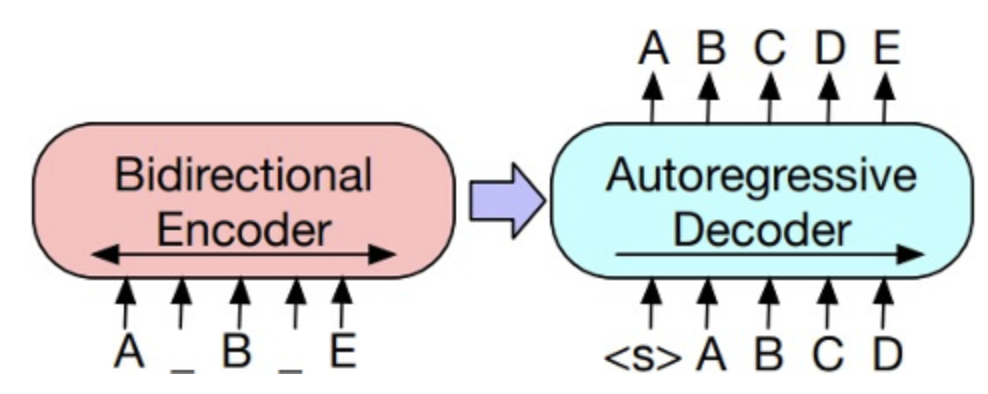
\includegraphics[width=7cm, height=2.5cm]{figures/BART}
%\caption{Encoder decoder model}
%%\Description{autoencoder}
%\label{fig:TL}
%\textcolor{red}{Notes: the figure will be replaced with a new figure}
%\end{figure}


BART has three big components: 1) noise transformation, 2) bidirectional encoder, and 3) autoregressive decoder.
i.	Noise transformation happens right before the encoder. Noise transformation will add some noises onto the inputs before feeding the data into the encoder. Having such action is to prevent the overfitting problem. There are five ways of corrupting the input: Token Masking, Sentence Permutation, Document Rotation, Token Deletion, and Text Infilling. The authors examined all of them and found that BART with text infilling could give the most consistently strong performance.
ii.	Next, the corrupted data will feed into the encoder that is able to read in both directions. This encoder produces a set of hidden states that capture the meaning and context of the input text.
iii.	Lastly, the set of hidden states will then get pushed to the autoregressive decoder that reads from left to right. This decoder basically generates a probability distribution over all possible tokens, given the hidden states and the masked input text. It then samples a token from the distribution and appends it to the output text in a step-by-step manner, where each token is conditioned on the previously generated tokens.

One reason why we choose BART is that it has richer documentation on how users can do fine- tuning and feed their own dataset to suit their own needs, compared to other novel pretrained models. Also, BART can establish abstractive summarization which is our objective. The evidence shown in the paper is highly abstractive with only a few phrases copied from the input.



\subsubsection{Transfer Learning in BART}
As mentioned above, BART hasn’t been trained on any long conversation dataset that includes multiple speakers. We plan to feed some of the AMI and ICIS corpus to BART and utilize another portion of the data to validate the outcome.

We are using transfer learning to train our model. In transfer Learning we need select a baseline model which acts as the source model, and we fine-tuned using the dataset. For each of the experiments we evaluated the experiment outcomes using both qualitative and quantitative metrics which are discussed in the nest section.

For faster prototyping, we used the HuggingFace Trainer API which allows us to use train models and save the best. The Trainer API also allows us to use TensorBoard to evaluate the training and evaluation performances. Once uploaded to HuggingFace, we can utilize the instant Inference API to use our model for demos.


\begin{figure}[thpb]
	\centering
	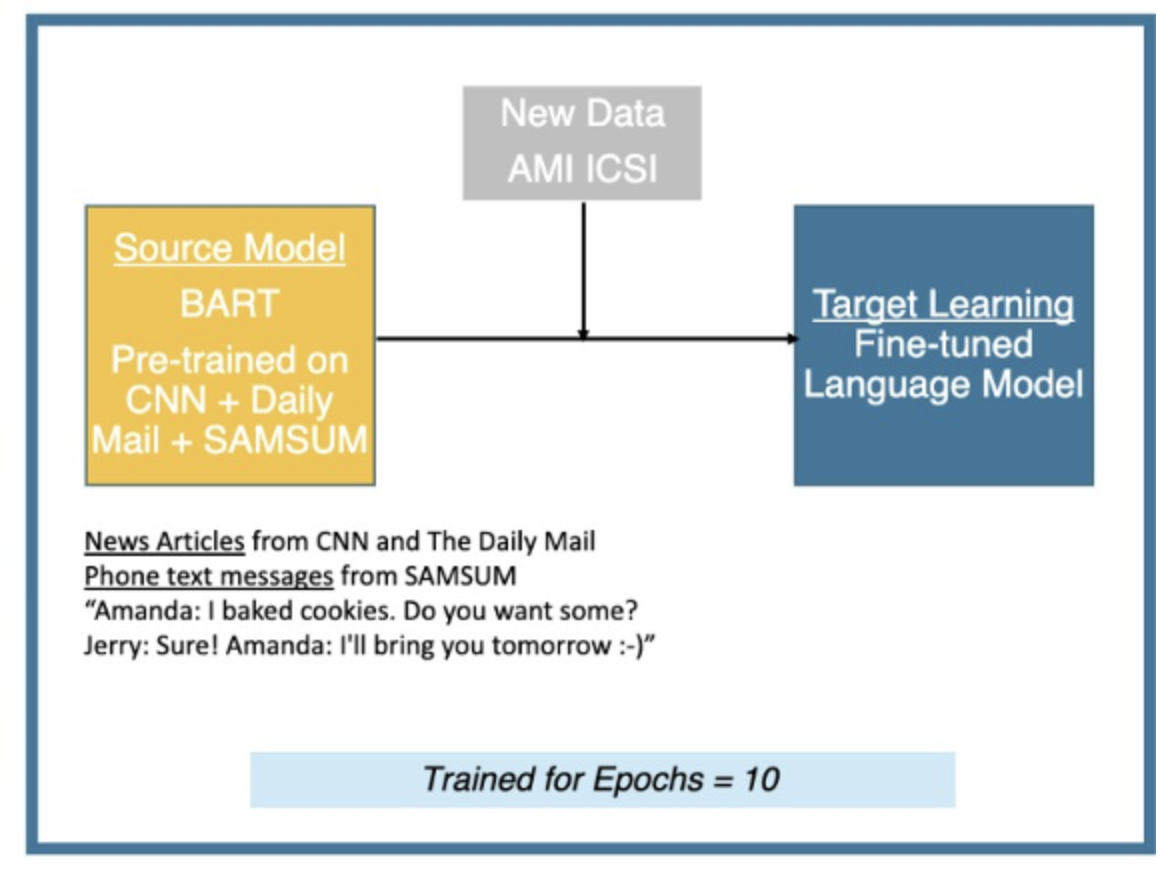
\includegraphics[width=7cm, height=4.5cm]{figures/TL}
	\caption{Transfer learning model}
	%\Description{autoencoder}
	\label{fig:TL}
	\textcolor{red}{Notes: the figure will be replaced with a new TL}
\end{figure}


\subsection{User Interface}
The application consists of two pages, with the first page dedicated to transcription and the second to summarization. Starting with the first page, at the top of our user interface, we offer the browse and upload buttons for users to locate and upload their local files. A clear button is also provided to reset the current application state to the initial state, enhancing visibility.

Beneath these buttons, we offer a transcription box that contains the transcribed content from the audio file. The transcription box enables users to edit the transcribed content if they find it necessary to change a word, number, or sentence. The reason for providing such editing functionality is that the accuracy of converting audio to text heavily depends on the quality of the microphone input.

Currently, our system is unable to identify speaker names mentioned in any conversation for accurate speaker labeling. Therefore, below the transcription box, we provide a table with the first column displaying the speaker tags identified by our system, and the second column allowing users to change the corresponding speaker tags to names of their choice. To apply all changes made, a change button is provided next to the table. We also provide a download link that allows users to download the updated transcript if they wish to save it locally.

At the bottom of our user interface, we incorporate an audio player and display an unmodifiable original content box, allowing users to listen and track the progress. Users can hover over and click on any point in the timeline, and the audio player will automatically jump to the selected time.

Navigating to the second page of our application, users can read the summary of the updated transcript. To obtain the system-generated summary, users must click the "Get my summary" button to initiate the summarization process. After a certain amount of processing time, the summary will appear in the box located below the button. Lastly, keywords from the meeting are also provided. These keywords are extracted from the transcription box on the first page. Arranged from top to bottom, the first list contains single words, the second list contains pairs of words, and the third list contains groups of three consecutive words. These keywords are offered to help users better comprehend the conversation.

\textcolor{red}{Need to explain the methods for user interface \& figures???. its above in black }

\vspace{15mm}




%
%\begin{algorithm}[tphb]
%%	\setstretch{1.6}
%	\caption{ANVO($D_{train}$, $k_{min}$, $k_{max}$, $\epsilon$)} \label{alg:sampling1}
%	\begin{algorithmic}[1]
%		\STATE \textbf{Input: } 
%	$D_{train}$ is a set of number of class-labeled training data points, $k_{min}$ is the minimum $k$ value for  $KNN$ search, $k_{max}$ is the maximum $k$ value, $\epsilon$ is the value to add to each attribute of the generated data point if the average difference is equal to the zero vector.  \\
%		\STATE \textbf{Output:} A balanced training dataset augmented by synthetic data\\ 
%		\STATE \textbf{Method:}
%		\STATE Split $D_{train}$  into majority class dataset ($MA$) and minority class dataset ($MI$) and record their number of instances as $N_{MA}$ and $N_{MI}$, respectively.  
%		\STATE $N_{syn} \leftarrow N_{MA} - N_{MI}$
%		\IF{If $k_{max} > N_{MI}-1$} \STATE $k_{max} \leftarrow N_{MI}-1$
%		\ENDIF
%		\IF{If $k_{min} \geq k_{max}$} \STATE $k_{min} \leftarrow \lceil\frac{k_{max}}{2}\rceil$
%		\ENDIF
%		\STATE Initailization: $S \leftarrow \{\}$, $i \leftarrow 1$, $\overrightarrow{avg_{diff}} \leftarrow $ 0 for all attributes in $D_{train}$, $\overrightarrow{avg_{diff}}$ is the average vector of the differences between the selected minority data point and its $k$ neighbors
%		\REPEAT
%			\STATE $P \leftarrow $ Choose a random minority data point %that has not already used all the possible $k$ values to generate data, save as point
%			\STATE $k \leftarrow $ Choose a random integer in the range $[k_{min}, k_{max}]$ that has not already been used with the point $P$ to generate data
%			\STATE Find the $k$ nearest neighbors of $P$ using $MI$ as the search space
%			\STATE $\overrightarrow{avg_{diff}} \leftarrow $ obtain a vector that represents the average difference between $P$ and its $k$ neighbors. 
%			\STATE $P_{new} \leftarrow $ Generate a new data point, $P_{new} = P + \overrightarrow{avg_{diff}}$
%			\IF{$\overrightarrow{avg_{diff}} = \vec{0}$}
%				\STATE $P_{new} \leftarrow = P + \overrightarrow{\epsilon}$ 
%			\ENDIF
%			\STATE $S \leftarrow$ add ${\P_{new}}$
%		\UNTIL{$i \leq N_{syn}$, If there are still possible data points left to generate (i.e., all the minority points have not used all the possible $k$ values to  generate data)
%		}
%	    \STATE $D_{train} \leftarrow D_{train} + S$
%	    \STATE return $D_{train}$, this is a balanced training data augmented by minority class synthetic data
%	\end{algorithmic}
%\end{algorithm}





%\begin{center}
%	\begin{figure*}
%		%	\widefigure
%		\begin{center}
%			\begin{subfigure}{0.35\textwidth}
%				\includegraphics[width=7.6cm, height=4.65cm]{figures-quan/LR1}
%				\caption{LR}
%				\label{fig:first}
%			\end{subfigure}  
%			\hspace{20mm}
%			\begin{subfigure}{0.35\textwidth}
%				\includegraphics[width=7.6cm, height=4.65cm]{figures-quan/LR2}
%				\caption{NN-based TL + LR}
%				\label{fig:second} 
%			\end{subfigure} \\
%			\vspace{5mm}
%			\caption{Model performance summary of 19 individuals: LR vs. NN-based TL + LR}
%			\label{fig:TLLR} 
%		\end{center}
%	\end{figure*}
%\end{center}
%
%

%\begin{equation}
%	\label{eq:eq1}
%	Exposure(x_i, t) = \sum_{j=1}^{N}E_i * t_{j, i}:
%\end{equation}
%
%math equation example in \ref{eq:eq2}. 
%
%\begin{math}
%	\label{eq:eq2}
%	\pi^{'}(\theta) = \pi(\theta|D)
%\end{math}
%by Bayes' formula.
%
%More examples are in \ref{eq:eq3}. 
%
%\begin{eqnarray}\label{hyper-update}
%	V_i^* & = &\frac{V_i}{1+c_iV_i} \label{eq:eq4}\\
%	m_i^* &= &\left(\frac{m_i}{V_i}+c_i\overline{t_i}\right)\frac{V_i}{1+c_iV_i} \label{eq:eq5}\\
%	% m_i^* &= &\left(\frac{m_i}{V_i}+c_i\overline{t_i}\right)V_i^*\\
%	a_i^* &= &a_i + \frac{c_i}{2}  \label{eq:eq6} \\
%	b_i^* &= &b_i + \frac12\left[\frac{m_i^2}{V_i}+\left(\sum_{r = 1}^{c_i}t_{i,r}^2\right)-\frac{{m_i^*}^{2}}{V_i^*}\right]  \label{eq:eq3}
%\end{eqnarray}








\section{Experiments}
\label{exp}


\subsection{Datasets} 
\label{sec:datasets} 

AMI corpus and ICSI corpus are publicly available datasets that contain 100 hours and 70 hours of meeting conversations recorded respectively. The duration of the audio files is between 20 minutes to 1 hour and 30 mins and there are 169 files in total. All the files are in
.wav format. The audio files consist of recording of multiple speakers interacting in workplace meeting.


AMI Corpus \cite{AMIurl, kraaij2005ami}, Augmented Multi-party Interaction Project, funded by the European Commission. 
ICSI Corpus \cite{ICSIurl, janin2003icsi}, International Computer Science Institute Speech Group, UC Berkley.
Reference Summary - Yale-LILY/QMSum: Dataset for NAACL 2021 paper: "QMSum: A New Benchmark for Query-based Multi-domain Meeting Summarization" (github.com)

We are also using reference summaries to train the model. The reference summaries are made by humans for the same meetings found in the AMI and ICSI corpus and are in text-format. The summaries are around a paragraph in length with 80 to 150 words.


\subsubsection{Data Preprocessing}

The audio files are relatively clean but quite lengthy, each conversation is around 50 mins long. One difficulty that we are facing is the length of the audio files. We are relying on OpenAI’s Whisper to transcribe the audio files and also using pyannote to diarize the sudio before combine the two to create the complete transcript. We used 1-GPU for carrying out the processing on the audio files. It takes approximately 3 mins. With 1-GPU to generate a transcript for a audio file that is 50 mins to 1 hour long.

\subsubsection{Exploratory Data Analysis}

Because we are dealing with NLP, we do not perform traditional data analysis. However, because the format of our dataset was not suitable for Summarization tasks, we had to perform data wrangling procedures.

i.	Errors in Transcription using Whisper
Due to the fact that we did not specify a specific language for the Whisper model, it was inferring languages from accents. This caused several errors in the transcriptions where Whisper switched to another language before reverting to English.

ii.	Data Wrangling
A typical dataset for summarization will have at least three columns: id, original text, and reference summary. However, since our dataset is a transcription of audio corpuses, we had to find reference human summaries. Fortunately, we were able to find reference summaries for the ICSI and AMI datasets.

Next, we had to combine all three features together so that they will be readable by HuggingFace’s Dataset API. We created a Python function to combine the meeting id, dialogue, and reference summary together and wrote them to a single JSON file. In other words, each JSON object is an individual meeting.


\subsection{Experiment Setup}
\subsubsection{System setup}

The following are some of the experiments that we setup:

\begin{itemize}
\item Changing the baseline model:
We attempted to use a baseline model without the pretraining on SAMSUM. However, the summary that the model produced was unsatisfactory for our purposes.

\item Different number of training epochs: 
We attempted to increase the number of epochs to ten for the second model. However, after the first epoch, the validation loss continues to increase and our HuggingFace model automatically saved the model from the first epoch.

\item Code is available in a public Github repository: \\https://github.com/vmarklynn/parrot. To setup the project environment please refer to $project\_setup.md$ file on Github which has instructions to setup all the dependencies for the proposed pipeline. Links to Models on Hugging Face are below:

	\begin{itemize}
	\item https://huggingface.co/vmarklynn/bart-large-cnn-samsum-icsi-ami
	\item https://huggingface.co/vmarklynn/bart-large-cnn-samsum-icsi-ami-v3
	\end{itemize}

\end{itemize}


\subsubsection{Performance Metrics}


Our evaluations on the performance of models are based on two types of evaluation methods: (1) Gnerated Length (GEN Len) and (2) Recall-Oriented Understudy for Gisting Evaluations (ROUGE).


 Gen Len measures the average length of the model-generated sequences. It is used to evaluate how well a language generation model can produce output of the desired length.

ROUGE compares automatically produced summaries against reference summaries which are human produced. For example, if a model produces a summary of ``the cat was found under the bed,” it is compared against ``the cat was under the bed.” In order to use ROUGE evaluations, there must be reference summaries by humans. In our experiments, we used datasets that include their summaries doen by humans \textcolor{red}{[reference]}.
%However, we have found previous human summaries for our data set as mentioned above in the dataset section. 
ROUGE calculates three following metrics: %(1) Precision: how much of the model summary was relevant? (2) Recall: how much of the reference summary is recovered from the reference? (3) $F_1$-score: it symmetrically represents both precision and recall in one metric. Calculations details are as follows: 

\begin{itemize}
	
	\item Precision: how much of the model summary was relevant? Precision = Number of overlapping N-grams / Number of tokens in the generated Text
	
	\item Recall: how much of the reference summary is recovered from the reference? Recall = Number of Overlapping N-grams / Number of tokens in the reference Text
	
	\item $F_1$-score: it symmetrically represents both precision and recall in one metric. $F_1$-score = (2 * Precision * Recall) / (Precision + Recall)
	
\end{itemize}

In our analysis, we used three ROUGE methods:

\begin{enumerate}
\item Rouge-N: This measures the overlap between the generated text and the reference text in terms of n-grams. To compute the Rouge-N score,

	\begin{enumerate}[label=\roman*.]
	\item Tokenize the generated text and the reference text into n-grams of size N.
	\item Compute the number of overlapping n-grams between the generated text and the reference text.
	\item Compute the precision, recall, and F1-score using the formulas above. 
	\end{enumerate}


\item Rouge-L: This measures the overlap between the generated text and the reference text in terms of longest common subsequences. To compute the Rouge-L score,


	\begin{enumerate}[label=\roman*.]
	\item Tokenize the generated text and the reference text into individual words.
	\item Compute the longest common subsequence between the generated text and the reference text.
	\item Compute the precision, recall, and F1-score using the following formulas:
	\end{enumerate}


\item Rouge-Lsum: It computes the Rouge-L score for multiple sentences, and then averages the scores. In other words, Rouge-Lsum is the same as Rouge-L, but it is calculated at the document level, considering all sentences together, rather than calculating it per sentence and then averaging the scores.

\end{enumerate}

A good Rouge-1 score typically falls between 40 and 50, while a Rouge-L score of around 30 or higher is generally considered good \textcolor{red}{[ref]}. However, these metrics have limitations as they primarily focus on the syntactical overlap and disregard semantic aspects. For instance, if the model effectively rewords and restructures the original text, Rouge scores might not fully capture its performance. To overcome these limitations, it is beneficial to involve multiple experts with diverse backgrounds who are skilled at summarizing. By incorporating their feedback along with the performance metrics, the quality of the output generated by the model can be significantly enhanced. This approach offers a more comprehensive evaluation that considers both syntactical and semantic aspects of summarization.



%\begin{figure}[thpb]
%	\centering
%	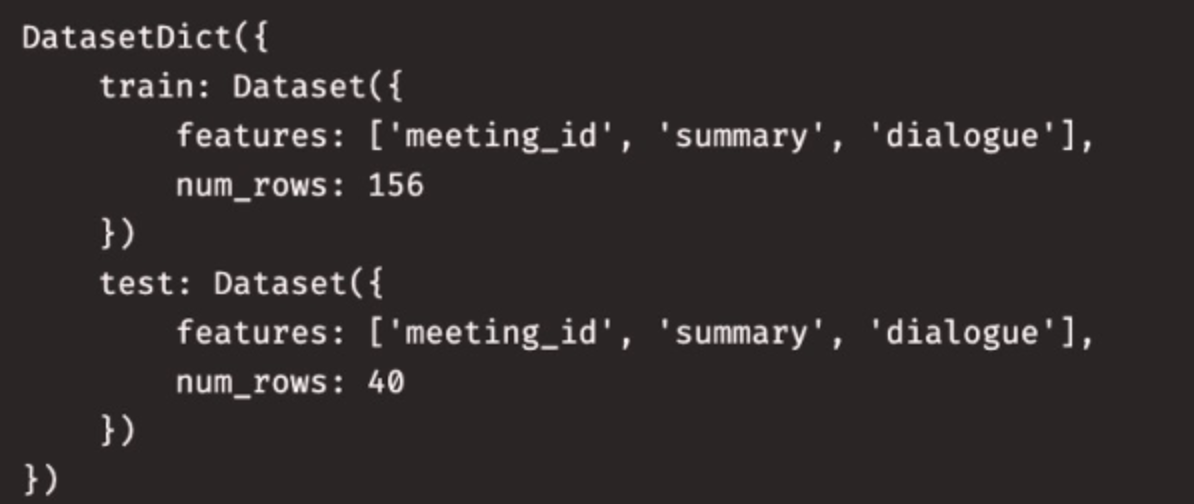
\includegraphics[width=8cm, height=3cm]{figures/JSON}
%	\caption{Example of JSON format}
%	%\Description{autoencoder}
%	\label{fig:TL}
%	\textcolor{red}{Notes: the figure will be replaced with a new TL}
%\end{figure}



\subsection{Quantitative Analysis}

\textcolor{red}{!!! This section needs more work to analyze the results. Any other results for quantitative analysis?}

In this section, we compare two BART models: (1) BART-A: It was trained on the CNN Daily Mail and SAMSUM dataset and retrained the model with our datasets using HuggingFace's Trainer API. This model is suitable for summarizing articles and short chat messages as it was trained. However, it may not produce good summaries for long dialogues \textcolor{red}{[reference?]}. Our quantitative results throughout the epochs are shown in the table below:


%\begin{figure}[thpb]
%	\centering
%	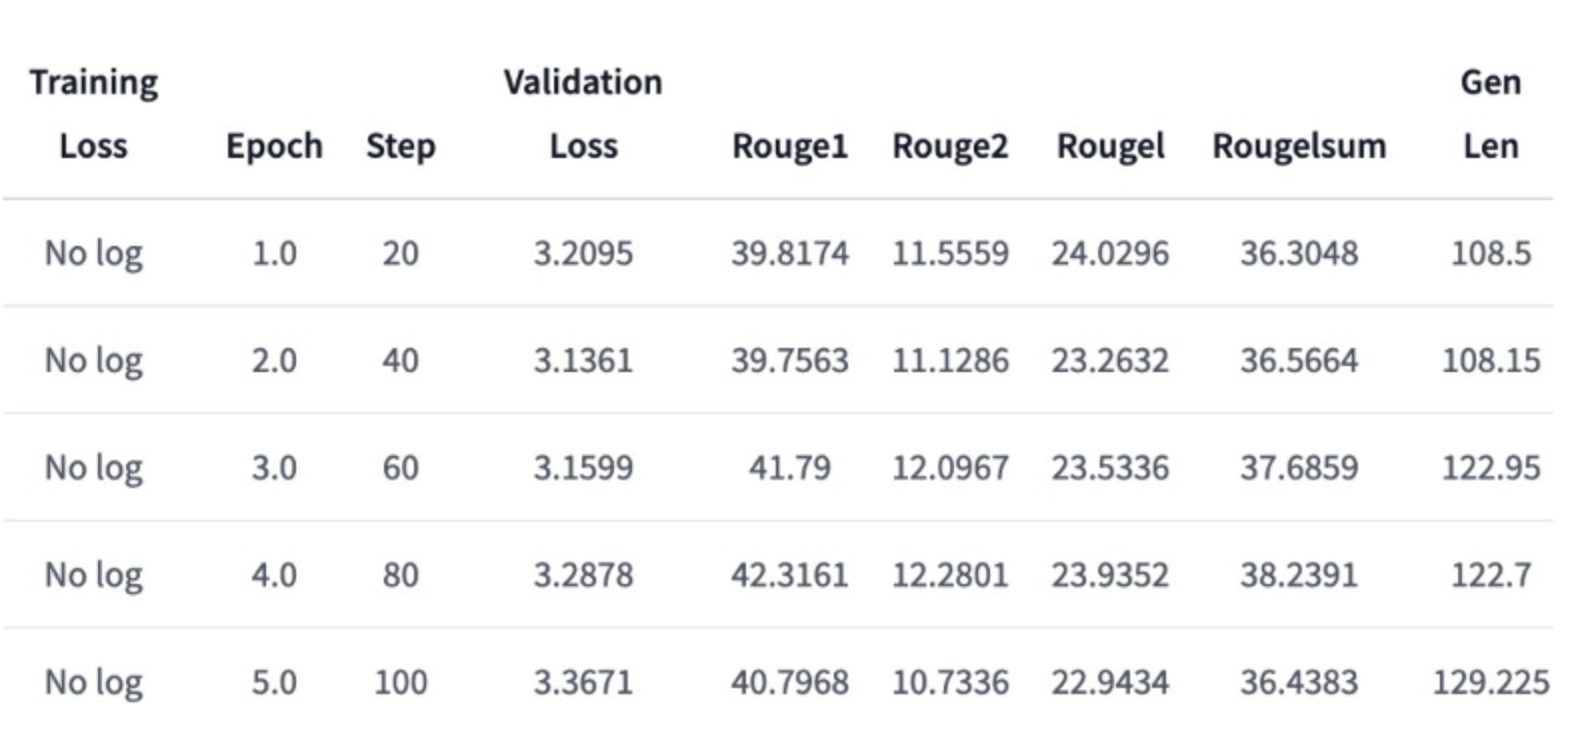
\includegraphics[width=8cm, height=3cm]{figures/res1}
%	\caption{1st model}
%	%\Description{autoencoder}
%	\label{fig:TL}
%	\textcolor{red}{Notes: the figure will be replaced with a table}
%\end{figure}

%
%\begin{table*}[h]
%	\caption{Hyperparameters in model retraining}
%	\label{tab:hyperparam}
%	\begin{center}
%		\begin{tabular}{l|l|l|l|l|l|l|l|l}
%			\hline
%			Epoch & Step & Training loss  & Validation loss & Gen Len & Rouge-1 & Rouge-2 & Rouge-L & Rouge-Lsum \\
%			\hline
%			1 & 20 & No log & 3.2095 & 108.503 & 39.817 & 11.556 & 24.030 & 36.305 \\
%			\hline
%			2 & 40 & No log & 3.1361 & 108.152 & 39.756 & 11.129 & 23.263 & 36.566 \\
%			\hline
%			3 & 60 & No log & 3.1599 & 122.954 &  41.790 & 12.097 & 23.534 & 37.686 \\
%			\hline
%			4 & 80 & No log  & 3.2878 & 122.701 & 42.316 & 12.280 & 23.935 & 38.239 \\
%			\hline
%			5 & 100 & No log & 3.3671 & 129.233 & 40.797 & 10.734 & 22.943 & 36.438 \\
%			\hline
%		\end{tabular}
%	\end{center}
%\end{table*}


\textcolor{red}{What is the difference between Modal-A and Model-B? The second model must have different training, right?}

\textcolor{red}{Need to explain the model performance results}



\begin{table*}[h]
	\caption{Model performance comparison}
	\label{tab:hyperparam}
	\begin{center}
		%\begin{tabular}{l|l|l|l|l|l|l|l|l|l}
			\begin{tabular}{r|r|r|r|r|r|r|r|r|r}
			\hline
			Model & Epoch & Step & Training loss  & Validation loss & Gen Len & Rouge-1 & Rouge-2 & Rouge-L & Rouge-Lsum \\
			\hline
			BART-A & 1 & 20 & No log & 3.2095 & 108.503 & 39.817 & 11.556 & 24.030 & 36.305 \\
			\cline{2-10}
			& 2 & 40 & No log & 3.1361 & 108.152 & 39.756 & 11.129 & 23.263 & 36.566 \\
			\cline{2-10}
			& 3 & 60 & No log & 3.1599 & 122.951 &  41.790 & 12.097 & 23.534 & 37.686 \\
			\cline{2-10}
			& 4 & 80 & No log  & 3.2878 & 122.704 & 42.316 & 12.280 & 23.935 & 38.239 \\
			\cline{2-10}
			& 5 & 100 & No log & 3.3671 & 129.233 & 40.797 & 10.734 & 22.943 & 36.438 \\ 
			\hline
			\hline
				BART-B & 1 & 135 & No log & 3.2308 & 185.794 & 38.427 & 13.646 & 22.366 & 35.235 \\
		\cline{2-10}
		& 2 & 270  & No log & 3.3026 & 146.853 & 40.175 & 11.794 & 23.266 & 36.472 \\
		\cline{2-10}
		& 3 & 405  & No log & 3.5199 & 141.765 & 39.821 & 12.162 & 22.777 & 36.497 \\
		\cline{2-10}
		& 4 & 540  &  2.2131 & 4.0508 & 131.441 & 40.433 & 11.655 & 22.996 & 36.878 \\
		\cline{2-10}
		& 5 & 675  &  2.2131 & 4.6988 & 145.971 & 38.410 & 9.831 & 20.389 & 34.197 \\
		\cline{2-10}
		& 6& 810  &  2.2131 & 4.9590 & 169.245 & 38.576 & 9.634 & 20.865 & 35.032 \\
		\cline{2-10}
		& 7 & 945 & 2.2131 & 5.4264 & 148.039 & 38.281 & 9.576 & 21.141 & 34.599 \\
		\cline{2-10}
		& 8 & 1080 & 0.4010 & 5.4887 & 139.353 & 38.301 & 9.688 & 21.240 & 34.158 \\
		\cline{2-10}
		& 9 & 1215 & 0.4010 & 5.8044 & 145.235 & 39.960 & 10.433 & 22.690 & 36.241 \\
		\cline{2-10}
		&10 & 1350 & 0.4010 & 5.8987 & 138.794 & 39.093 & 10.841 & 21.914 & 35.507 \\
			\hline
		\end{tabular}
	\end{center}
\end{table*}



\begin{table*}[h]
	\caption{Hyperparameters in model retraining}
	\label{tab:hyperparam}
	\begin{center}
				\begin{tabular}{l|l|l|l|l|l|l|l}
							\hline
							Model & learning rate & train batch size & eval batch size &seed & optimizer&LR scheduler type & \# epochs \\
							\hline
							BART-A &  5e-05  &  8 & 8 & 42& Adam, $\beta=(0.9, 0.999), \epsilon=1e-8$& linear & 5 \\
							\hline
							BART-B &  5e-05  &  1 & 1 & 42& Adam, $\beta=(0.9, 0.999), \epsilon=1e-8$& linear & 10 \\
							\hline
						\end{tabular}
			\end{center}
\end{table*}

Table \ref{tab:hyperparam} summarizes hyperparameters we used for the two models. 

%\begin{figure}[thpb]
%	\centering
%	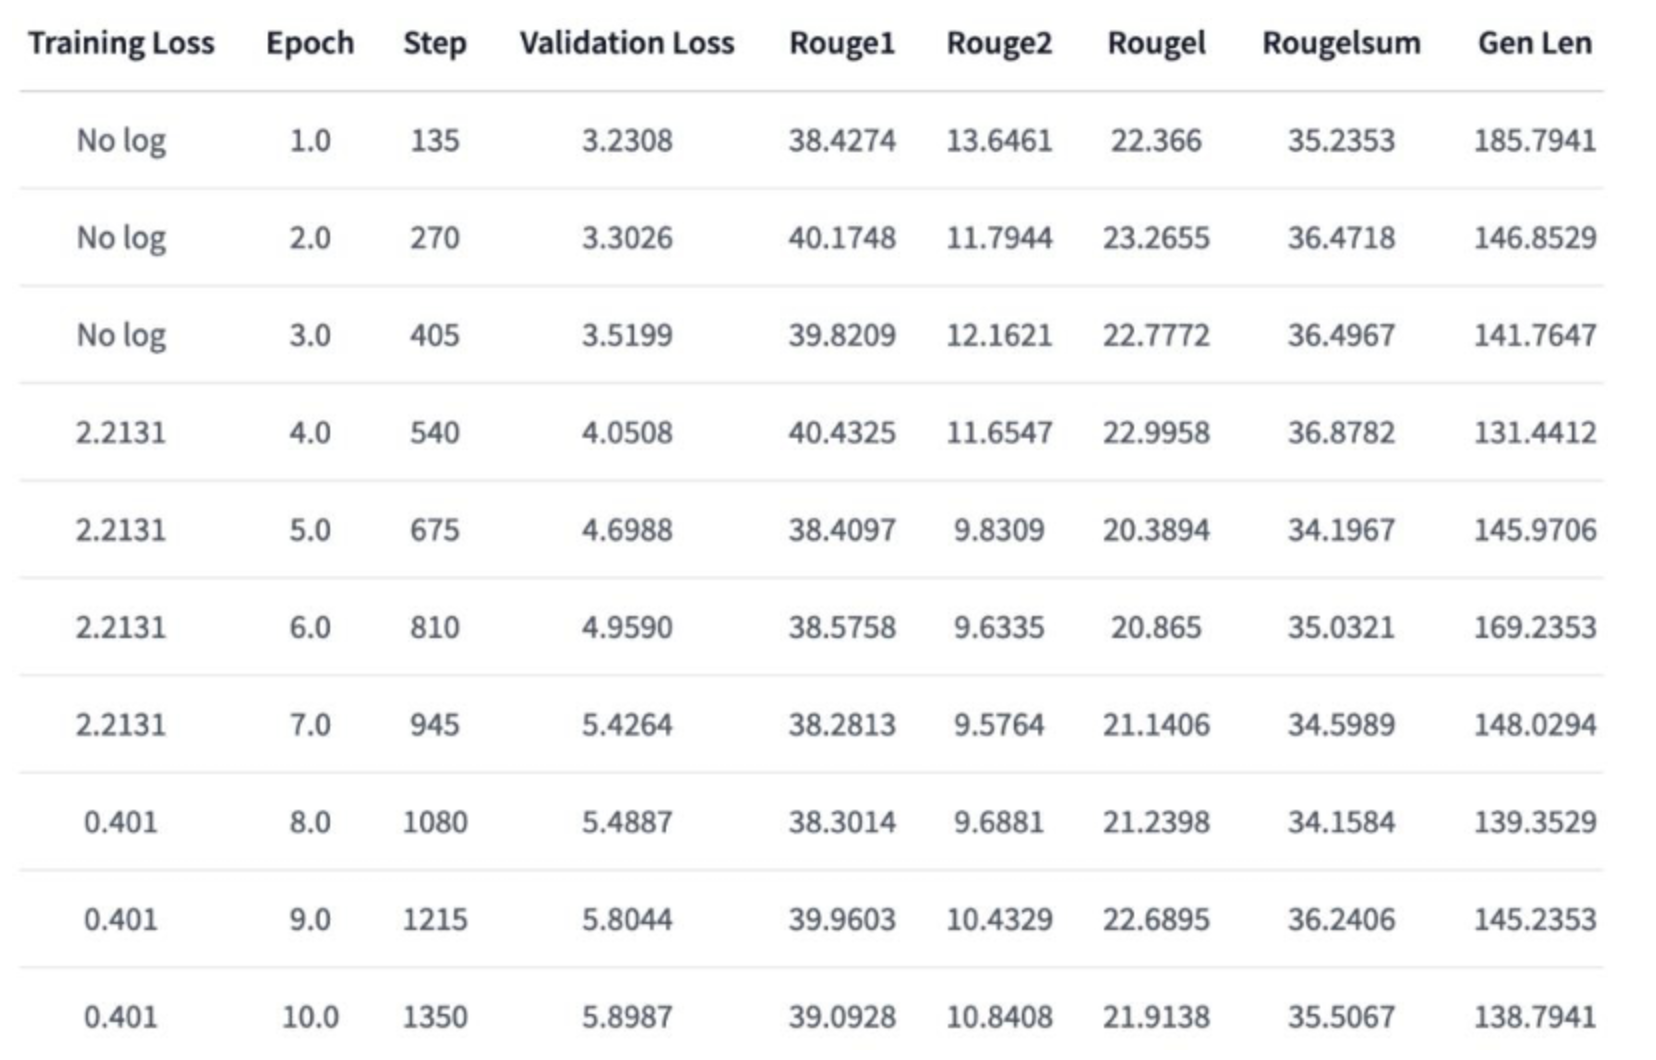
\includegraphics[width=9cm, height=4cm]{figures/res2}
%	\caption{2nd model}
%	%\Description{autoencoder}
%	\label{fig:hyperparam}
%	\textcolor{red}{Notes: the figure will be replaced with a table}
%\end{figure}


\subsection{Qualitative Analysis}

\textcolor{red}{!!! This section needs more work to analyze the results.}

This section presents qualitative results of our proposed pipeline using the BART-B model

We compared to the human reference summary. The output from our model is more comprehensive, accurately identifying the specific locations visited by the individuals. Summaries from BART-B and their corresponding summaries by humans are shown in  Table 3 . 


\begin{table*}[h]
	\caption{Qualitive analysis}
	\label{tab:matrix}
	\begin{center}
				\begin{tabular}{l|l|l}
							\hline
							Type & Machine Summary & Human Reference Summary    \\
							\hline
						Short prose/dialogue & The whole vacation was spent in Paris with my parents. &  \#Person1\# asks Person2\# what \#Person2\# did during  \\
						\textcolor{red}{[ref]}  & 	\textbf{They saw the Eiffel Tower, Nortre-Dame Cathedral, }   & the vacation to Paris.  \#Person2\# saw \textbf{all the most} \\
						&	\textbf{the Seine River, and the famous art museums.} They & \textbf{famous places and enjoyed sitting in cafes most.}  \\
						&	also went a a boat tour around the city, and they had & \#Person1\#'s looking forward a vacation. \\
						&\textbf{a lot of fun sitting in cafes and watching people.}  & \\
							\hline
					Long meeting & This is the \textbf{first meeting of the new remote control}& Manager gave the team members \textbf{a brief introduction} \\
					 \textcolor{red}{[ref]}    & \textbf{project.} Project Manager introduced the team members & \textbf{of the new remote control project}, then the team \\\
					 & to each other and the project manager. The team first  & \textbf{\textcolor{cyan}{started an ice breaking game by drawing their }}  \\
					 & \textbf{\textcolor{cyan}{got acquainted with each other by drawing their}} & \textbf{\textcolor{cyan}{animals. The expected selling price of the remote}} \\
					 & \textbf{\textcolor{cyan}{favourite animals.}} Next, the team discussed the &  \textbf{\textcolor{cyan}{is 25 Euros}} and the production costs would be limited \\
					 & working design of the remote control device. They & to twelve and a half Euro per unit. Marketing plan \\
					 & decided to \textbf{\textcolor{green}{make it more user-friendly}} than the  & would depend on overhead costs. The team agreed that \\
					 & previous one, so they made some changes to the design. & the remote needs to be robust, and they wanted \textbf{\textcolor{green}{it to be}} \\
					 & \textbf{\textcolor{cyan}{The final product would be a remote control with }} & \textbf{\textcolor{green}{a device for all with accessible buttons}}. Project \\
					 & a fancy look, \textbf{\textcolor{green}{ease of use}}, and \textbf{\textcolor{cyan}{cost 25 Euros}}. & Manger suggested it to be only a television remote \\
					 & & control instead of a multi-functional one. \\
					 \hline
					 A meeting of & \multicolumn{2}{l}{Machine Summary (no human reference summary)}\\
					 Load of the Rings & \multicolumn{2}{l}{\textbf{The meeting began with the forging of the Great RINGS, each set with a single GEN, which were given}} \\
					\textcolor{red}{[ref]}   & \multicolumn{2}{l}{\textbf{to the Dwarf Loards, great miners, and craftsmen of the  mountain halls.} Next, the meeting moved onto} \\
					 & \multicolumn{2}{l}{a discussion of the design of the New Line Cinema's next project, which was due to be presented in the next} \\
					 & \multicolumn{2}{l}{meeting. Then, the group moved onto the discussion of how they would govern each other and their own lives. } \\
					 & \multicolumn{2}{l}{\textbf{They discusssed how they could make the best use of the power they had, and decided that they would}} \\
					 & \multicolumn{2}{l}{\textbf{have to be more like the KINGS of Men.} Finally, they talked about how to make the project a success. The} \\
					 & \multicolumn{2}{l}{meeting ended with a brief discussion of their next meeting} \\
					 \hline
						\end{tabular}
			\end{center}
\end{table*}



%\begin{figure}[thpb]
%	\centering
%	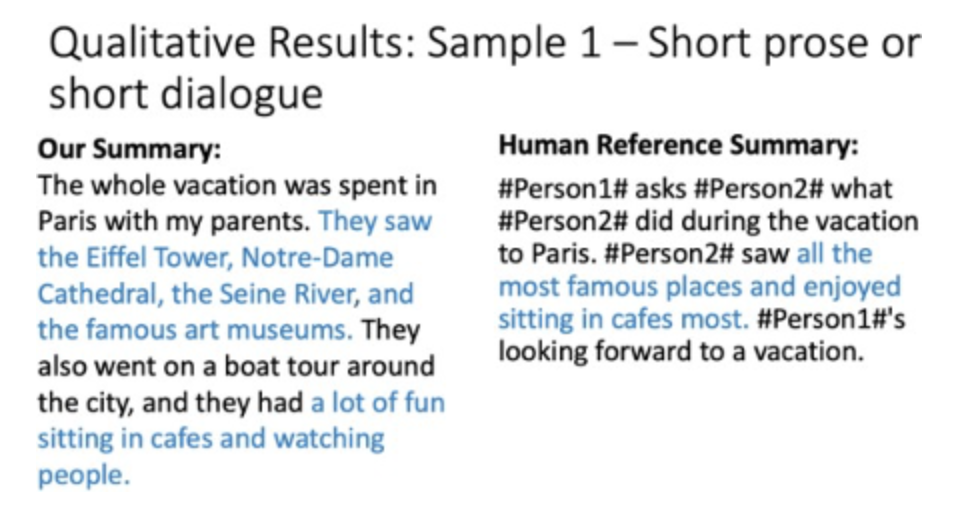
\includegraphics[width=8cm, height=3cm]{figures/q1}
%	\caption{Short prose or dialogue comparison}
%	%\Description{autoencoder}
%	\label{fig:q1}
%	\textcolor{red}{Notes: the figure will be replaced with a table}
%\end{figure}



Our model covers about 60 percent of the content of the reference summary and performs well in most parts. However, in the second sentence, the phrase 'project manager' is unnecessarily repeated at the end.

%
%\begin{figure}[thpb]
%	\centering
%	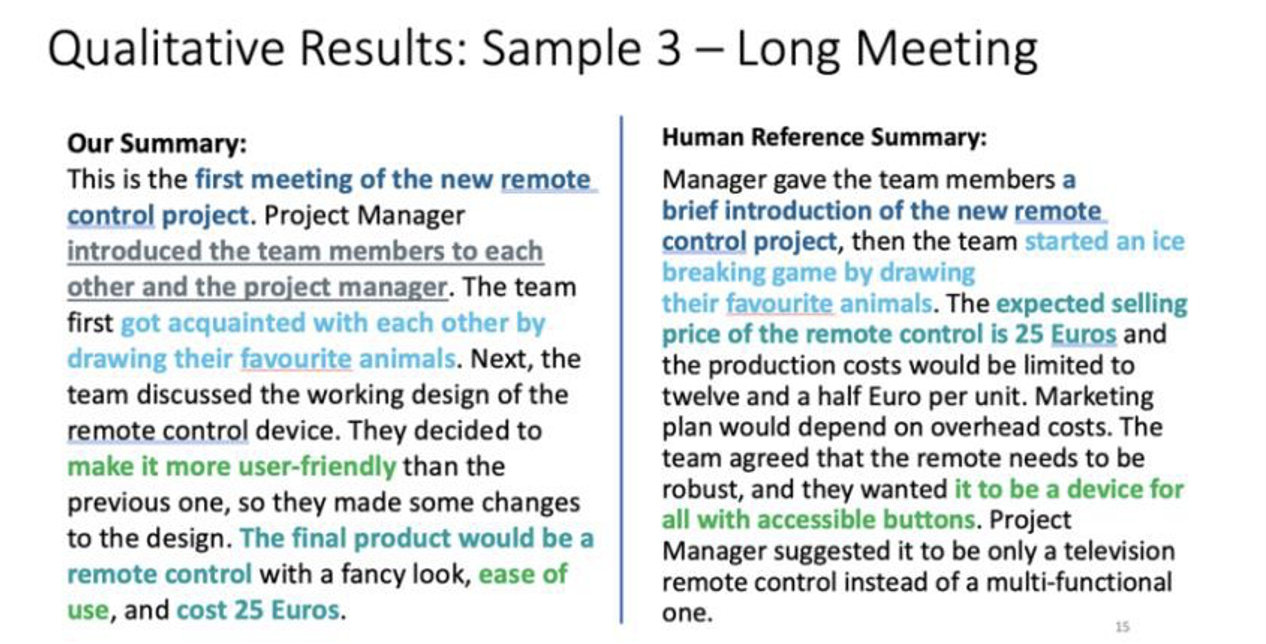
\includegraphics[width=8cm, height=3cm]{figures/q3}
%	\caption{Long meeting summarization comparison}
%	%\Description{autoencoder}
%	\label{fig:q3}
%	\textcolor{red}{Notes: the figure will be replaced with a table}
%\end{figure}







We tested the limits of our model by giving input of the entire Lord of the Rings screenplay to summarize. It has been able to provide a reasonable summary but as one can see it makes a wrong inference that people should be more like the KINGS of Men when they shouldn’t because the KINGS of Men become corrupted by power. We can also see that the model has learned typical workplace lingo such as “The meeting began …” and “They discussed …” due to the transfer learning and finetuning we have carried out.

%\begin{figure}[thpb]
%	\centering
%	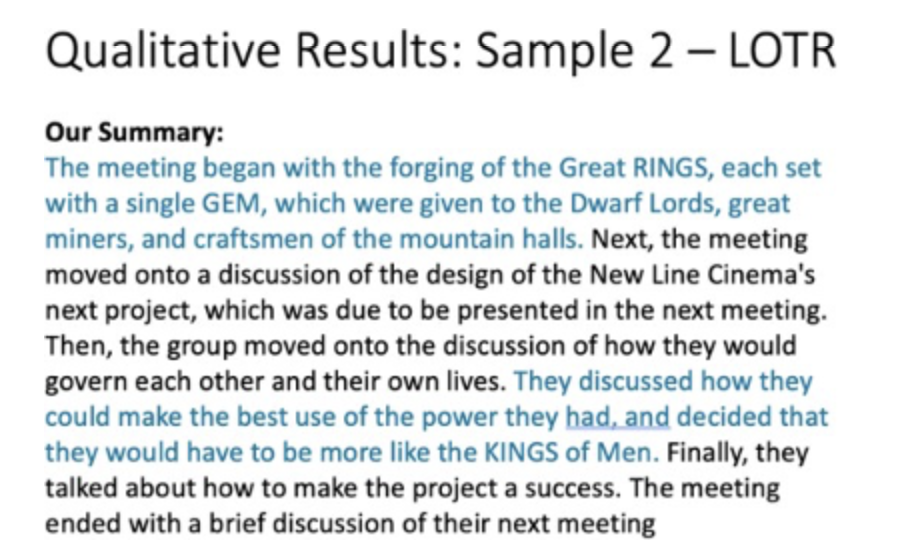
\includegraphics[width=8cm, height=3cm]{figures/q2}
%	\caption{Summarization of Lord of the Rings complete screenplay}
%	%\Description{autoencoder}
%	\label{fig:q2}
%	\textcolor{red}{Notes: the figure will be replaced with a table}
%\end{figure}



%
%\begin{table}[h]
%	\caption{Confusion matrix}
%	\label{tab:matrix}
%	\begin{center}
%			\begin{tabular}{l|l|l|l|l}
%					\hline
%					Metric & IoU Score  & Precision & Recall & F1 Score   \\
%					\hline
%					Average &  0.4111   &  0.555 & 0.856 & 0.710   \\
%					\hline
%				\end{tabular}
%		\end{center}
%\end{table}


%
%\begin{table}[h]
%	\caption{A ligher model for edge computing}
%	\label{tab:matrix}
%	\begin{center}
%		\begin{tabular}{l|l|l|l|l}
%			\hline
%			Model & Classification  & Accuracy & File Size	 & Latency   \\
%			\hline
%			EfficientNet0.tflite&	Pothole	&0.9955	 & 21 MB&	< 15 MS \\
%			&	Normal Road	& & &	 \\
%		\end{tabular}
%	\end{center}
%\end{table}

%\subsection{UI: Django Framework}




%\begin{figure*}[thbp]
%	\begin{center}
%		\mbox{
%			\subfigure[Sensitivity]{
%				\scalebox{0.5}[0.52]{\includegraphics*{figures/real_sen}}
%			}
%			\subfigure[Specificity] {
%				\scalebox{0.5}[0.52]{\includegraphics*{figures/real_spe}}
%			}
%		}
%			\mbox{
%		\subfigure[Precision]{
%			\scalebox{0.5}[0.52]{\includegraphics*{figures/real_pre}}
%		}
%		\subfigure[$F_1$-score] {
%			\scalebox{0.5}[0.52]{\includegraphics*{figures/real_f1}}
%		}
%	}
%		\caption{Performance improvement: LR vs. TL + LR classifiers with 5 SMOTE variants on asthma patients' datasets}
%		\label{fig:zone2}
%	\end{center}
%\end{figure*}
%


%
%\begin{table*}[tphb]
%	\caption{Average model performance of 19 individuals}
%	\label{tab:classification}
%	\begin{center}
%		\begin{tabular}{l|l|cccccc}
%			\hline
%			%\multicolumn{2}{l|}{Algorithm}  & weighted accuracy & sensitivity & specificity & precision & $F_{1}$ score  \\
%			Classifier & Sampling method & weighted accuracy & sensitivity & specificity & precision & $F_{1}$ score  \\
%			\hline
%			\hline
%			DT & \texttt{No up-sampling} & 	0.645& 0.614  &	0.679 &	0.607 &	0.596  \\
%			%\hline 
%			& \texttt{ROS} & 	\textbf{0.738} &	\textbf{0.727} &		\textbf{0.757} &	\textbf{0.687} & \textbf{0.741} \\
%			\hline 
%		\end{tabular}
%		\vspace{2mm}
%		\\ * SMOTE: the synthetic minority over-sampling technique  \cite{chawla2002smote}
%	\end{center}
%\end{table*}

%
%\begin{table*}[tphb]
%	\caption{Classifier performance measures on  asthma patients' datasets}
%	\label{tab:real}
%	\begin{center}
%		\begin{tabular}{l|l|c|cccc|c}
%			\hline
%			%\multicolumn{2}{l|}{Algorithm}  & weighted accuracy & sensitivity & specificity & precision & $F_{1}$ score  \\
%			Classifier & Sampling method & Weighted Acc. & Sensitivity & Specificity & Precision avg. & $F_1$ score avg.  & $S_{rank}$ \\
%			\hline
%			\hline
%			DT & \texttt{No oversampling} &   0.5801 (5) &	0.2780 (7)	&0.8822 (1)	&0.5821	(4) &0.5663 (6) &5.6 \\
%			%\cline{2-7} 
%			& \texttt{ROS} &  0.5779 (6) &	0.3369	(6) &0.8188	(2) &0.5738	(6) &0.5655 (7) &5.8  \\
%			& \texttt{SMOTE} &  0.5813 (5) &	0.3663 (5) &0.7963 (3) 	&0.5727 (6) 	&0.5692 (4)  & 4.8 \\
%			& \texttt{G-SMOTE} &  0.5851 (3)	&0.3781	(4) &0.7880 (6) 	&0.5838 (3) 	&0.5697 (3) & 3.8 \\
%			%& \texttt{ACOR-SMOTE} &  0.5977	&0.4790	&0.7165	&0.5761	&0.5648 \\
%			& \texttt{Gamma-SMOTE} &  0.5849 (4) &	0.3901 (2) &0.7797 (7)	&0.5798 (5)	&0.5677 (5) & 3.7  \\
%			& \texttt{SDD-SMOTE} &  0.5955 (1)	&0.3980 (1) &	0.7931 (5)	&0.5850	(2) &0.5773 (2)  & \textbf{1.8} \\
%			& \texttt{$^{*}$ANVO} &  0.5873	(2) &0.3803 (3) &	0.7944 (4) &	0.5891 (1) &0.5776 (1) & \textbf{2.3} \\			
%			\hline 
%			KNN & \texttt{No oversampling} & 	0.5443 (7)	&0.1279 (7)	&0.9607	(1) &0.5575	(7) &0.5195 (7)   &6.4\\
%			%\cline{2-7} 
%			& \texttt{ROS} & 0.5996	(5) &0.4742	(6) &0.7250	(2) &0.5792	(3) &0.5734 (1) &4.0\\
%			& \texttt{SMOTE} &  0.6188	(1) &0.5697	(1) &0.6679	(5) &0.5829	(1) &0.5673 (2) & \textbf{1.6} \\
%			& \texttt{G-SMOTE} &  0.6067 (2) &	0.5441	(3) &0.6692	(4) &0.5798	(2) &0.5635 (3) & \textbf{2.9}  \\
%			& \texttt{Gamma-SMOTE} &  0.5902 (6) 	&0.5262	(5) &0.6541	(7) &0.5666	(6) &0.5452 (6) & 5.6\\
%			& \texttt{SDD-SMOTE} &  0.6061	(3) &0.5500	(3) &0.6623	(6) &0.5783	(4) &0.5615 (4) & 3.7 \\
%			& \texttt{$^{*}$ANVO} &  0.6025	(4) &0.5601 (2) &0.6731	(3) &0.5768	(5) &0.5608  (5) & \textbf{3.3} \\			
%			\hline 
%			LR & \texttt{No oversampling} & 	0.5303 (7)	&0.0762	(7) &0.9844	(1) &0.4656	(7) &0.4864 (7) & 6.4 \\
%			& \texttt{ROS} &  0.6088 (6) &	0.5175 (5) &0.7002 (7)	&0.5716 (6) &0.5606 (6) &5.1 \\
%			& \texttt{SMOTE} &  0.6168 (5)	&0.5028 (6) &0.7308	(4) &0.5933 (3)	&0.5852 (2) &4.4 \\
%			& \texttt{G-SMOTE} &  0.6199 (3)	&0.5260	(3) &0.7338	(2) &0.5992 (1)	&0.5884 (1)  & \textbf{2.1} \\
%			& \texttt{Gamma-SMOTE} &  0.6215 (2) &	0.5195 (4) 	&0.7134 (5)	&0.5918 (4) 	&0.5812  (4) & 4.1 \\
%			& \texttt{SDD-SMOTE} &  0.6240 (1)	&0.5390 (1)	&0.7089 (6) &0.5894 (5) 	&0.5805 (5) & \textbf{3.1} \\
%			& \texttt{$^{*}$ANVO} &  0.6194 (4)	&0.5301 (2) &0.7315 (3)	&0.5971	(2)&0.5847 (3)  & \textbf{2.3} \\			
%			\hline 
%			NB & \texttt{No oversampling} & 	0.5383 (7)	&0.0987 (7)	&0.9778 (1)	&0.5024 (7)	&0.5019 (7) & 6.4  \\
%			%\cline{2-7} 
%			& \texttt{ROS} & 0.6072 (1) 	&0.5096	(1) &0.7048	(7) &0.5714	(6) &0.5608 (6) & 3.6 \\
%			& \texttt{SMOTE} &  0.5992 (4) 	&0.3783	 (5) &0.8201 (2)	&0.5995	(2) &0.5910  (1) & \textbf{3.3} \\
%			& \texttt{G-SMOTE} &  0.5935 (5)	&0.3921	(3) &0.7948	(6) &0.5880	(3) &0.5823 (3) & \textbf{3.3} \\
%			& \texttt{Gamma-SMOTE} & 0.5892 (6) 	&0.3761	(6) &0.8023	(5) &0.5838	(5) &0.5753 (5) & 5.5 \\
%			& \texttt{SDD-SMOTE} &  0.6011	(3) &0.3880	(4) &0.8141	(3) &0.6016	(1) &0.5876 (2) & \textbf{2.9} \\
%			& \texttt{$^{*}$ANVO} &  0.6028	(2) &0.3952	(2) &0.8103	(4) &0.5843	(4) &0.5822 (4) & \textbf{3.0}  \\			
%			\hline 
%		\end{tabular}
%		\vspace{2mm}
%		\\ *  indicates our new SMOTE variant. 
%	\end{center}
%\end{table*}
%


%
\section{Discussion}
\label{discussion}
We introduced a pipeline that transcribes, diarizes, and summarizes conversation meetings using Whisper, Pyannote, and a retrained BART model, resulting in a 148% improvement in summarization. Our solution is integrated into a user-friendly website built with Django, allowing users to upload meeting recordings and obtain comprehensive transcripts and summaries. Our work paves the way for more effective meeting analysis and information accessibility in various contexts and industries.

However, our project currently faces limitations in terms of the quality of the human reference and the availability of data. Expanding the scope and performance of our summarizer to cover different meeting domains requires access to more diverse and comprehensive data sets. This would enable the model to learn and adapt to various meeting scenarios, ultimately improving its accuracy and generalizability.

Future work should focus on making our application more marketable to companies by improving the summarization capabilities and providing accurate and insightful analysis of workplace meetings.
Additional application features could include visualizations of meeting using colors and waveforms, speaker recognition that allows the model to learn overtime to recognize previously encountered voices, and sentiment analysis.









%%
%% The acknowledgments section is defined using the "acks" environment
%% (and NOT an unnumbered section). This ensures the proper
%% identification of the section in the article metadata, and the
%% consistent spelling of the heading.
%\begin{acks}
%Acknowledgements go here
%\end{acks}

%%
%% The next two lines define the bibliography style to be used, and
%% the bibliography file.
\bibliographystyle{ACM-Reference-Format}
\bibliography{base}


%%
%% If your work has an appendix, this is the place to put it.
%\appendix



\end{document}
%\endinput
%%
%% End of file `sample-sigconf.tex'.
